\section{Máxima suma de ruta}

Problema 18 de Project Euler (\url{https://projecteuler.net/problem=18})

Al empezar en la punta del triángulo de abajo y moviéndose adyacentemente por los números de la fila inmediatamente abajo, la máxima suma de ruta que se obtiene desde la cúspide hasta la base es de 23.

\begin{figure}[h]
    \centering
    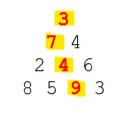
\includegraphics{Guia/triangulochico.jpg}    
\end{figure}

Esto es, 3+7+4+9=23

Enuentre la máxima suma de ruta (comenzando desde la cúspide y moviéndose en números adyacentes) del triángulo de abajo.

\begin{figure}[H]
    \centering
    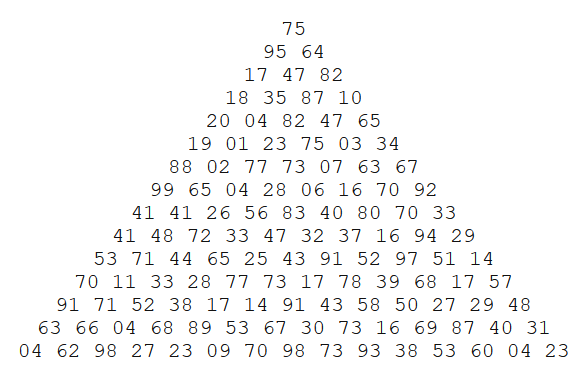
\includegraphics{Guia/triangulogrande.PNG}
\end{figure}

\paragraph{Nota:} Al existir sólo 16384 rutas, es posible resolver este problema al probar cada una de ellas. Sin embargo, el problema 67, tiene el mismo desafío con un triángulo de 100 filas y no puede ser resuelto por un método de fuerza bruta.

\paragraph{Pista:} Intente, en lugar de comenzar la iteración desde la cúspide del triángulo, comenzar desde la base. Con esto es más fácil encontrar el patrón de la ruta de máxima suma.